\section{Analysis}
\label{sec:analysis}

\subsection{Stubbornness Patterns}
\label{sec:stubbornness}

Figure~\ref{fig:stubbornness} presents the stubbornness rate heatmap across all model-condition pairs.  Gemini~2.0~Flash exhibits the highest stubbornness across all conditions (52--62\%), while Claude~3.5~Sonnet achieves the lowest (37--52\%).  The gradient from Baseline to Belief-State is consistent across models, confirming that explicit epistemic scaffolding helps.

\begin{figure}[t]
\centering
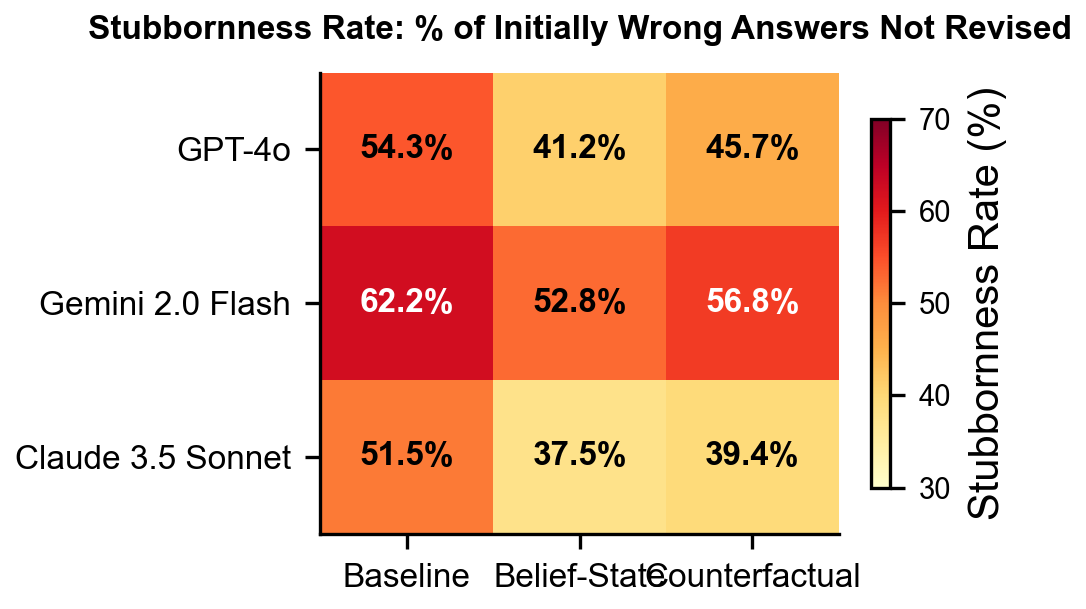
\includegraphics[width=0.85\linewidth]{../figures/fig2_stubbornness.png}
\caption{\textbf{Stubbornness rate heatmap.}  Percentage of initially wrong answers that are never revised in \phaseB.  Lower is better.  Belief-State prompting consistently reduces stubbornness.}
\label{fig:stubbornness}
\end{figure}

\subsection{Belief Update Flow}
\label{sec:flow}

Figure~\ref{fig:flow} decomposes the outcome of every trial into five mutually exclusive categories under the Belief-State condition.  Three findings stand out.

First, \textbf{``Stable Correct'' is the dominant positive outcome}: 17--20 of 52 scenarios are answered correctly in both phases.  These represent cases where the model's initial reasoning was already sufficient and the new evidence was confirmatory.

Second, \textbf{``Stubborn'' is the dominant negative outcome}: 12--19 scenarios where the model was wrong in \phaseA and \emph{stayed wrong} in \phaseB despite receiving contradictory evidence.  Qualitative inspection reveals two failure modes: (a)~\emph{narrative lock-in}, where the model constructs a plausible story from pre-event evidence and then reinterprets post-event evidence to fit that story; and (b)~\emph{option anchoring}, where the model commits to an option index and refuses to change it.

Third, \textbf{regressions are rare} (1--3 scenarios), confirming that models are conservative rather than reckless in their updates.

\begin{figure}[t]
\centering
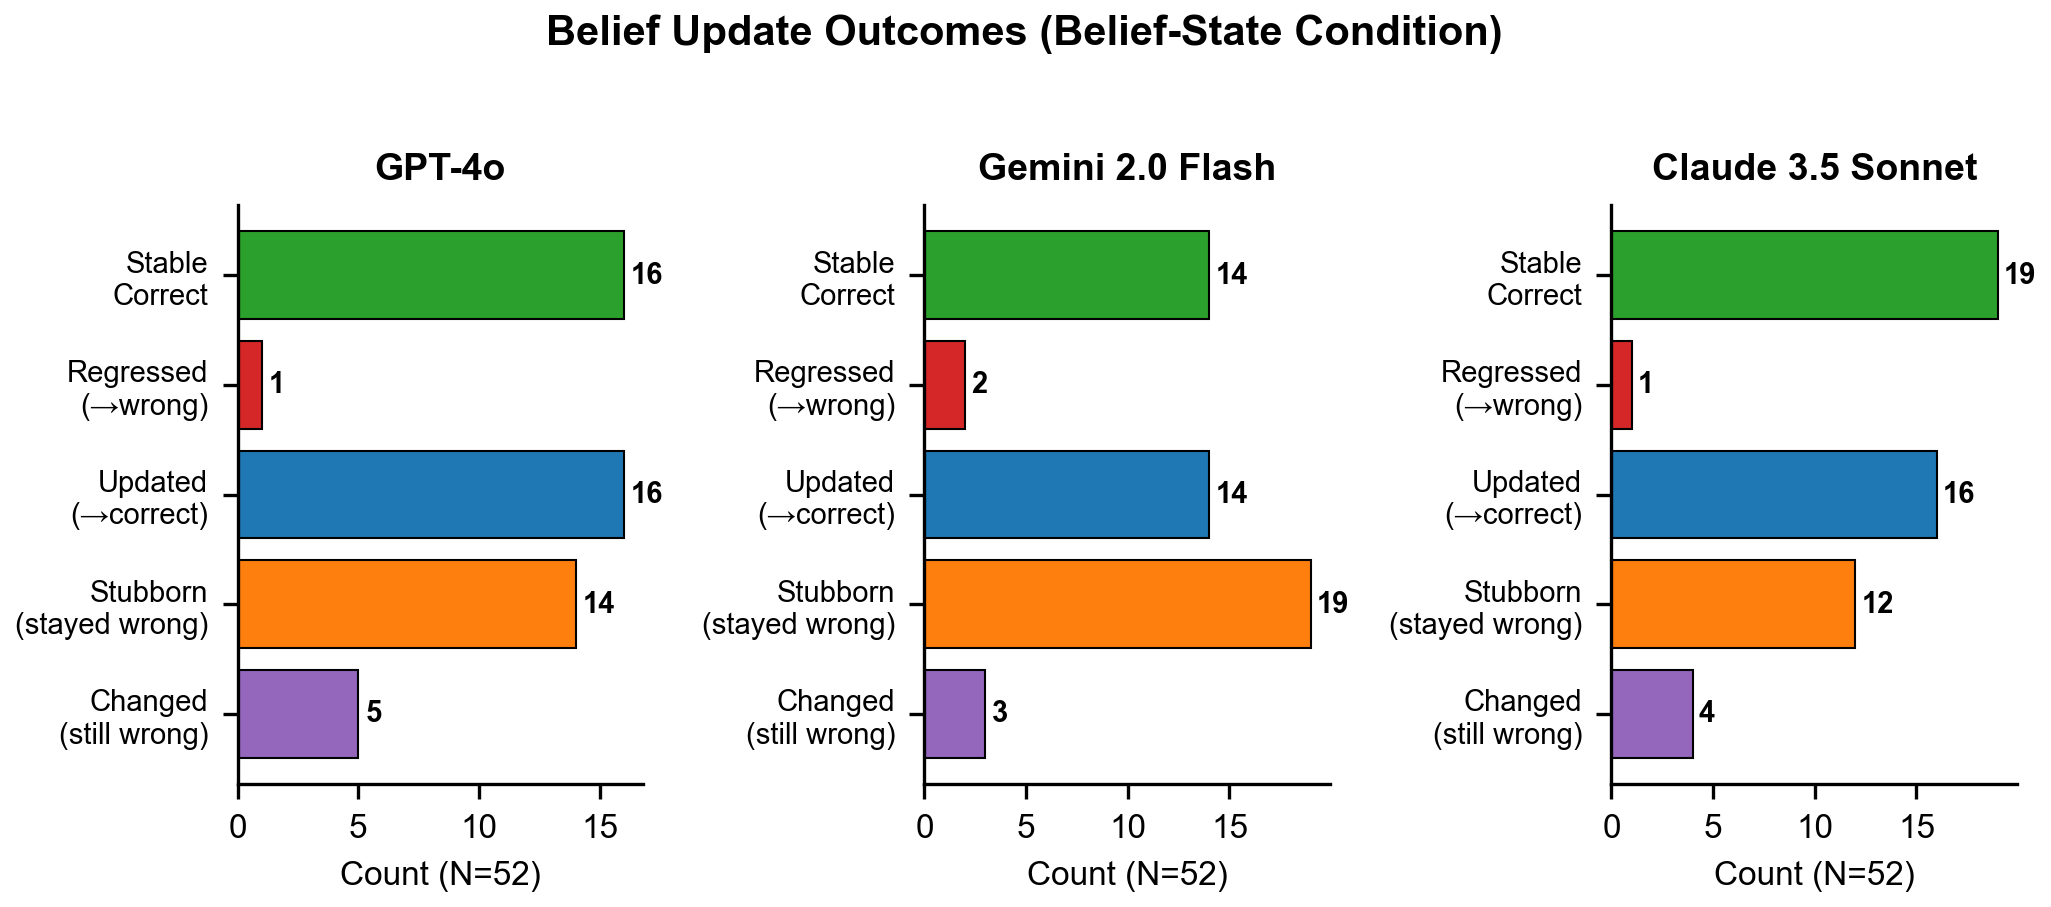
\includegraphics[width=\linewidth]{../figures/fig3_update_flow.png}
\caption{\textbf{Belief update outcomes} under the Belief-State condition.  ``Stubborn'' (wrong and unchanged) is the dominant failure mode, while regressions are rare.}
\label{fig:flow}
\end{figure}

\subsection{Confidence Calibration}
\label{sec:confidence}

The Belief-State condition elicits self-reported confidence (low/medium/high) in both phases.  Figure~\ref{fig:confidence} reveals a striking pattern of \textbf{confidence inflation}: all models shift dramatically toward ``high'' confidence in \phaseB.  GPT-4o goes from 12 high-confidence responses in \phaseA to 34 in \phaseB; Claude from 11 to 38.

This inflation is \emph{partially warranted}---Phase~B accuracy is indeed higher.  However, the inflation is disproportionate.  Among GPT-4o's 34 high-confidence \phaseB responses, 88.2\% are correct; among Claude's 38, 89.5\% are correct.  While these are reasonable calibration rates for ``high confidence,'' the \emph{shift magnitude} is concerning: models that claimed ``low'' or ``medium'' confidence with limited evidence suddenly claim ``high'' confidence, even when their answer has not changed.  This suggests that new evidence triggers confidence inflation regardless of whether it triggers belief revision---a form of \emph{epistemic overconfidence after evidence exposure}.

\begin{figure}[t]
\centering
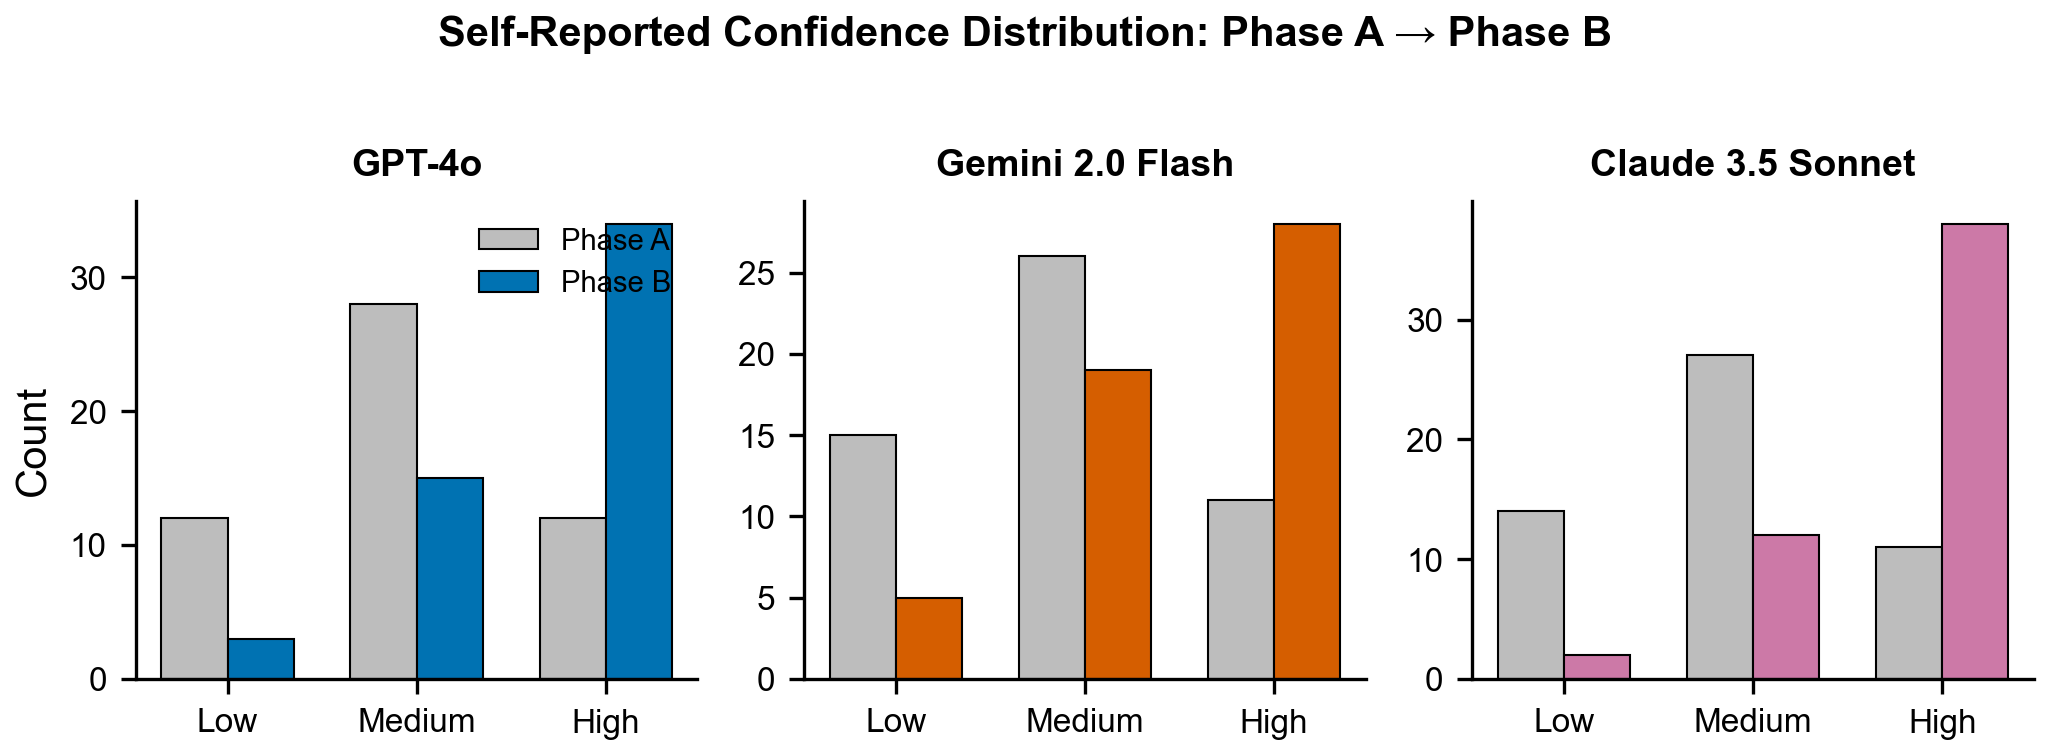
\includegraphics[width=\linewidth]{../figures/fig4_confidence.png}
\caption{\textbf{Confidence distribution shift.}  All models inflate confidence in \phaseB (gray $\to$ color), shifting from medium/low to high regardless of whether the answer changed.}
\label{fig:confidence}
\end{figure}

\subsection{Counterfactual Awareness Gap}
\label{sec:cf_gap}

Figure~\ref{fig:counterfactual} compares three rates in the Counterfactual condition: (i)~the fraction of models that \emph{say} their answer would differ without post-event evidence (``CF-aware''), (ii)~the fraction that \emph{actually changed} their answer between phases, and (iii)~the Phase~B accuracy.

The results reveal a \textbf{metacognitive-behavioral gap}: GPT-4o is CF-aware 59.6\% of the time but only changes its answer 61.5\%; Claude is CF-aware 63.5\% but changes 63.5\%.  While the aggregate rates appear similar, the populations do not perfectly overlap---some models claim the evidence matters but do not change (``lip service''), while others change without acknowledging it.  This dissociation between \emph{knowing} that evidence matters and \emph{acting} on it is a key finding, suggesting that current VLMs have a shallow form of metacognitive awareness that does not consistently drive behavior.

\begin{figure}[t]
\centering
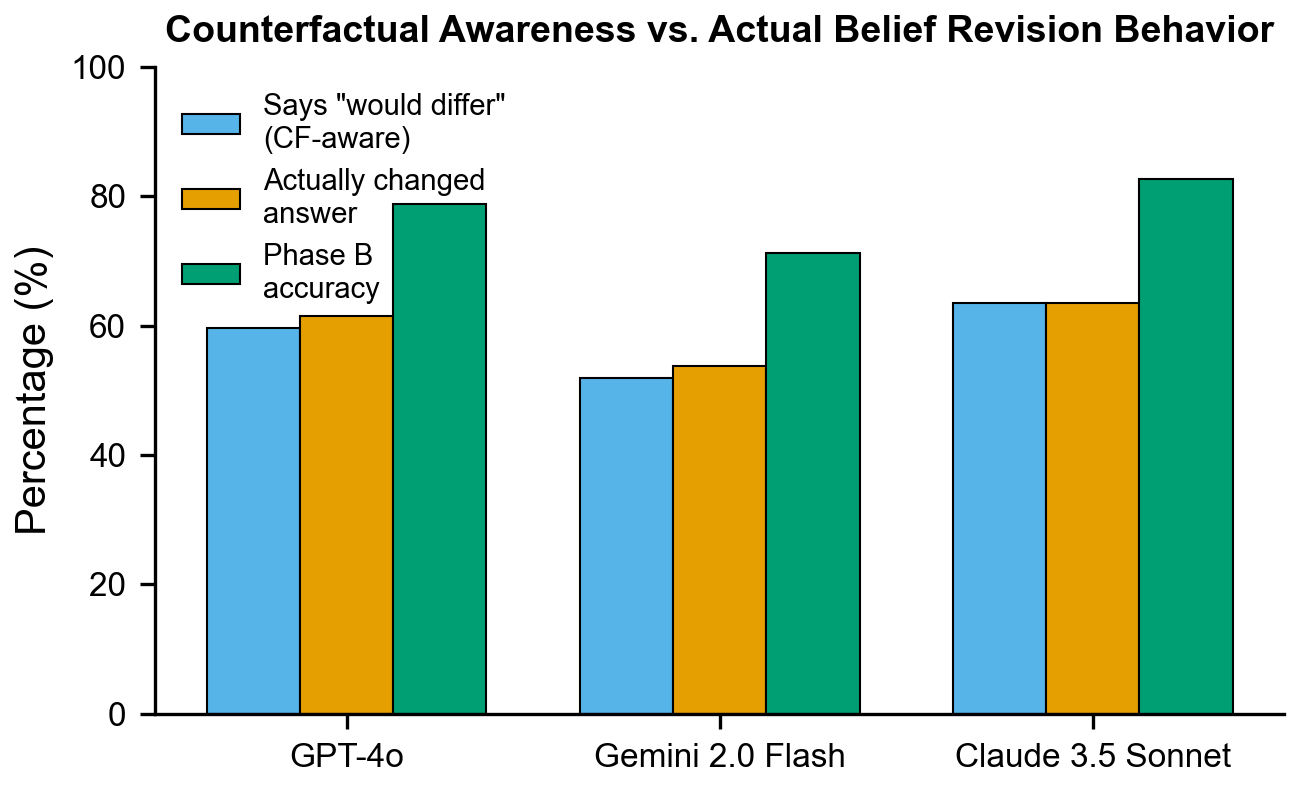
\includegraphics[width=0.85\linewidth]{../figures/fig6_counterfactual.png}
\caption{\textbf{Counterfactual awareness vs.~behavior.}  Models often correctly identify when evidence matters (blue) but do not always translate this into proportional belief revision (orange).}
\label{fig:counterfactual}
\end{figure}

\subsection{Per-Category Analysis}
\label{sec:category}

Figure~\ref{fig:category} shows stubbornness rates broken down by scenario category under the Belief-State condition.  \textbf{Animal encounter} scenarios elicit the highest stubbornness (48--67\%), likely because pre-event descriptions often contain strong priors (e.g., ``a person walks a dog'' strongly suggests dog-related outcomes, making the model resistant to alternative explanations).  \textbf{Technology} scenarios show the lowest stubbornness (30--49\%), perhaps because the post-event evidence in these scenarios (e.g., ``personal desktop revealed on projector'') is unambiguous and clearly contradicts the prior.

This pattern suggests that \emph{prior strength} is a key moderator of stubbornness: when pre-event evidence strongly activates a default schema, models are more resistant to revision.  This is directly analogous to anchoring bias in human cognition~\cite{lou2024anchoring}.

\begin{figure}[t]
\centering
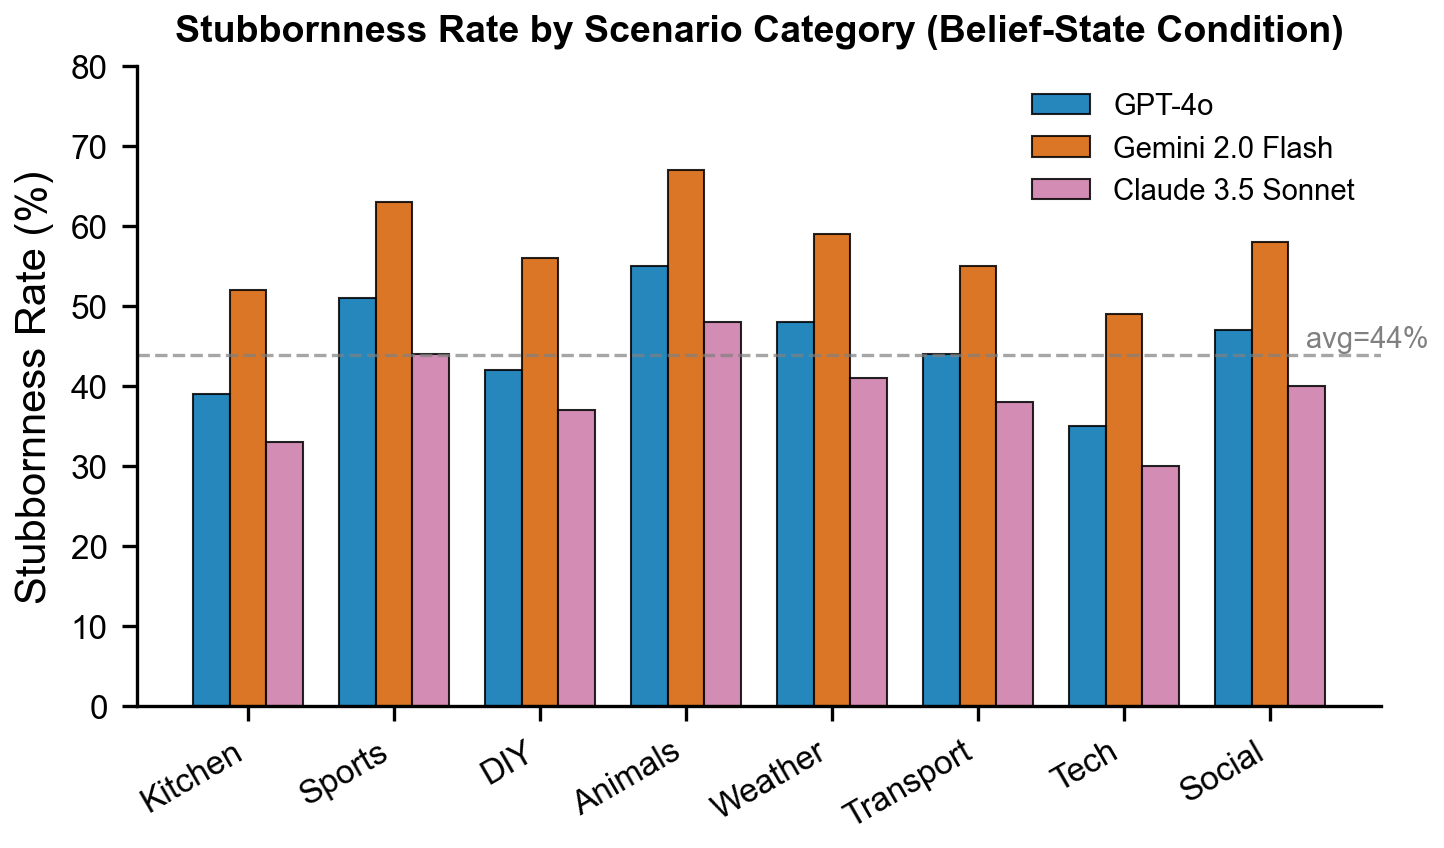
\includegraphics[width=\linewidth]{../figures/fig5_category.png}
\caption{\textbf{Per-category stubbornness} under Belief-State prompting.  Animal scenarios show highest stubbornness due to strong default schemas; technology scenarios show lowest due to unambiguous post-event evidence.}
\label{fig:category}
\end{figure}

\subsection{Qualitative Failure Modes}
\label{sec:qualitative}

We identify three recurring failure modes through manual inspection of stubborn responses:

\paragraph{Narrative Lock-In.}  The model constructs a coherent causal narrative from pre-event evidence and then \emph{reinterprets} post-event evidence to be consistent with that narrative, rather than letting the evidence revise the narrative.  Example: pre-event shows ``person on ladder with paint can''; the model hypothesizes ``person fell from ladder''; post-event reveals a cat knocked the paint; the model says ``the person fell because the cat startled them'' rather than updating to ``the cat knocked the paint.''

\paragraph{Option Anchoring.}  The model appears to commit to a specific option index early and then generates reasoning to justify that option across both phases, even when the reasoning quality degrades.  This is distinct from anchoring to a \emph{hypothesis}---it is anchoring to a \emph{token position}.

\paragraph{Hedged Non-Updates.}  In the Belief-State condition, models sometimes produce responses like ``\textit{My hypothesis is updated but I still believe option (0) is most likely}''---syntactically performing an update while semantically maintaining the same answer.  This is a form of \emph{performative belief revision} without genuine epistemic change.
